\begin{tikzpicture}
\node[anchor=south west,inner sep=0] (panel) at (0,0) {%
  \begin{minipage}[t]{0.34\linewidth}
    \IfFileExists{figures/ch01/ch01-06-site-schematic-brief.png}{%
      \begin{tikzpicture}
      \node[anchor=south west,inner sep=0] (img) at (0,0) {%
        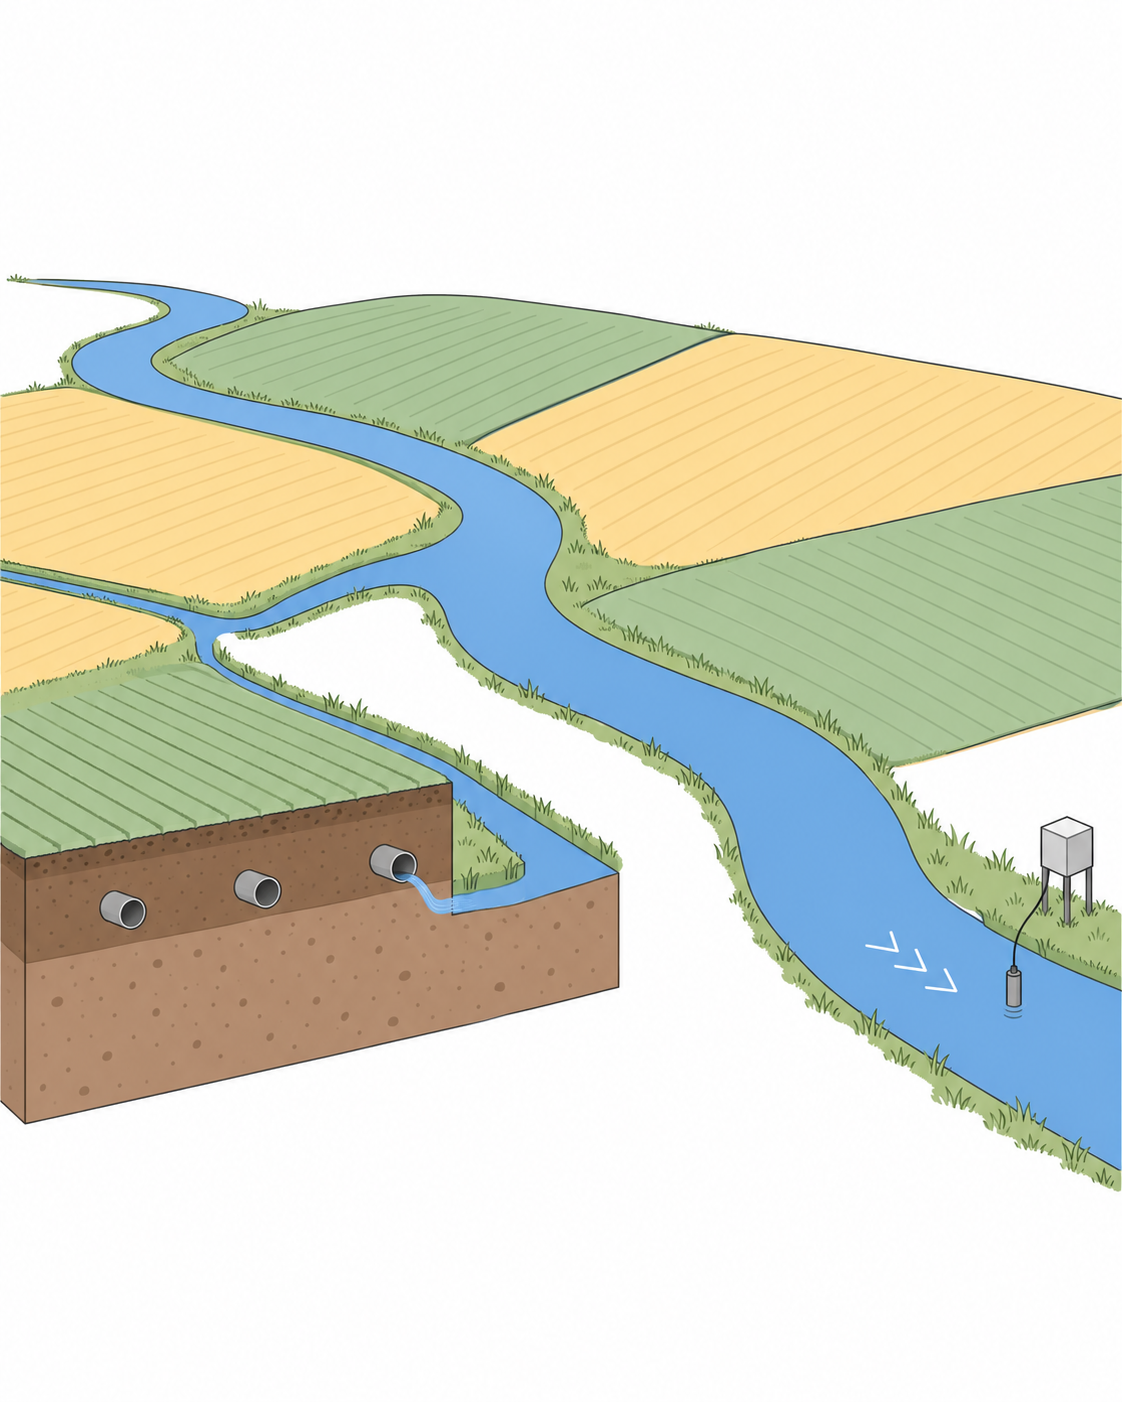
\includegraphics[width=\linewidth]{figures/ch01/ch01-06-site-schematic-brief.png}};
      \begin{scope}[x={(img.south east)},y={(img.north west)}]
        \tikzset{lbl/.style={font=\scriptsize,fill=white,fill opacity=0.8,text opacity=1,inner sep=1pt,align=center}}
        \node[lbl,text width=0.28,align=center] at (0.48,0.86) {农田（玉米—大豆，示意）};
        \node[lbl,text width=0.22,align=center] at (0.20,0.16) {地下排水管};
        \node[lbl,text width=0.18,align=center] at (0.10,0.44) {支沟};
        \node[lbl,text width=0.22,align=center] at (0.52,0.52) {Raccoon River};
        \node[lbl,text width=0.26,align=center] at (0.52,0.10) {监测站 USGS 05484500};
        \node[lbl] at (0.50,0.38) {水流方向};
      \end{scope}
      \end{tikzpicture}
    }{%
      \fbox{\parbox[c][0.36\linewidth][c]{0.34\linewidth}{\centering\scriptsize 缺少 ch01-06 底图\\（codex-image，未在本任务范围）}}
    }
    \par\vspace{1mm}{\scriptsize 示意，不按比例}
  \end{minipage}\hfill
  \begin{minipage}[t]{0.64\linewidth}
    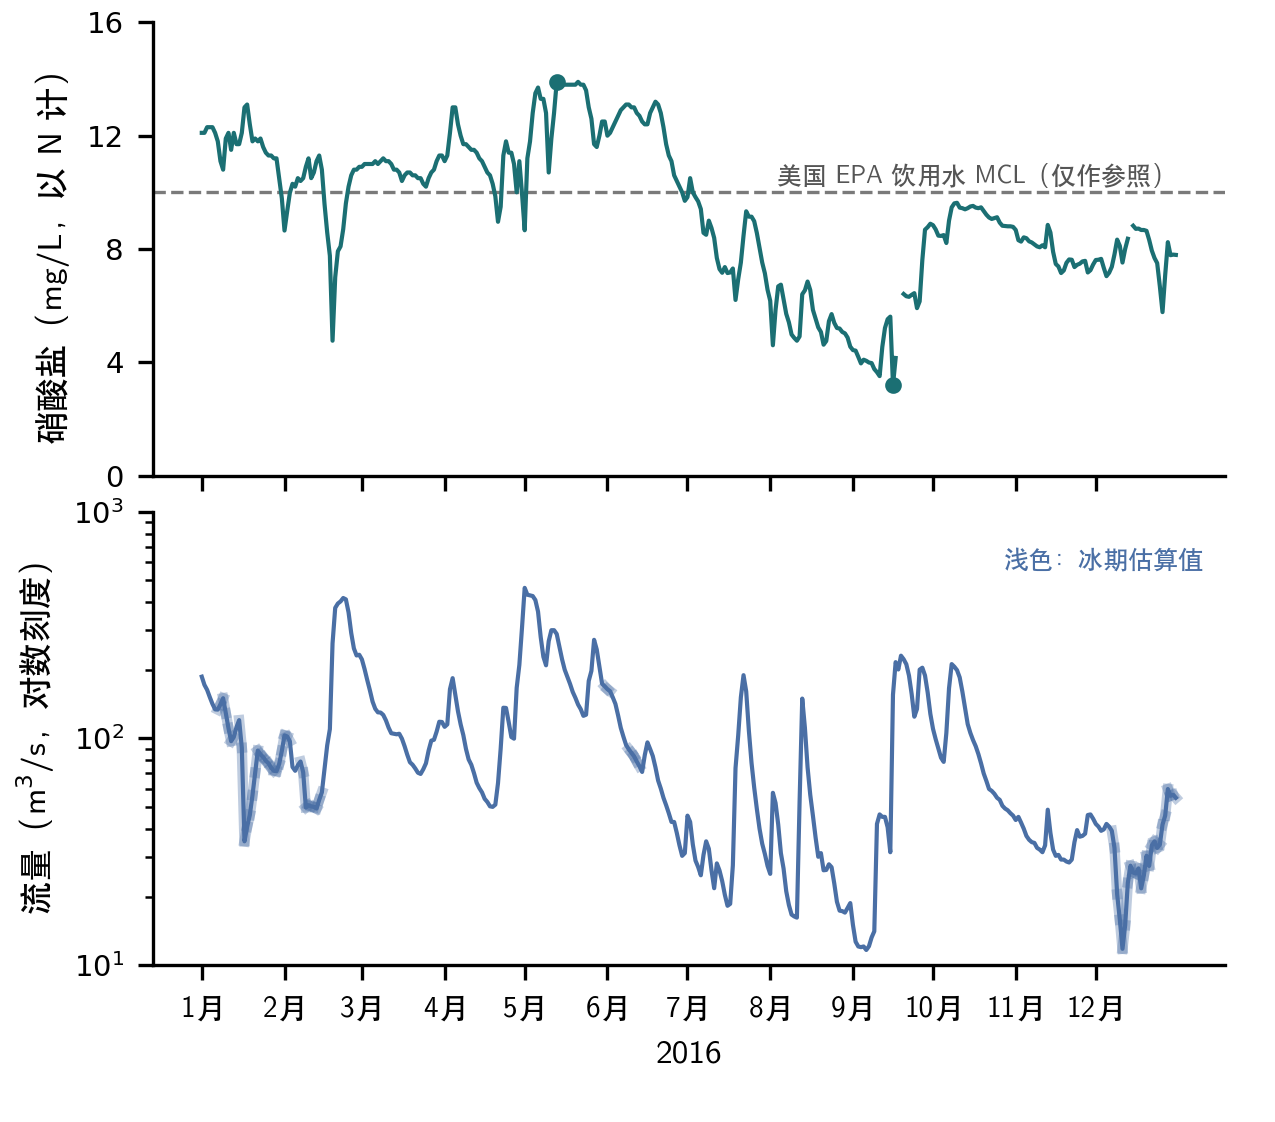
\includegraphics[width=\linewidth]{figures/ch01/ch01-04-nitrate-panel-brief-zh-panel.png}
  \end{minipage}};
\node[anchor=south west,font=\bfseries\small] at ([xshift=1mm,yshift=1mm]panel.north west) {a};
\node[anchor=south west,font=\bfseries\small] at ([xshift=0.34\linewidth,yshift=1mm]panel.north west) {b};
\end{tikzpicture}
